\section{Increasing Sparsity}
\label{sec:sparsity}

We noted that the 45 cluster spectral clustering result described in
the previous section assigned many more tags to each word than the
gold standard.  To quantify the difference we used a measure called
tag perplexity defined as follows:

\[ 2^{\frac{1}{N}\sum_{i=1}^N -\log_2 p(t_i | w_i)} \]

Here $N$ is the number of words in the corpus, $w_i$ is the i'th word,
$t_i$ is its assigned cluster or tag, and $p(t_i|w_i)$ is the fraction
of times word $w_i$ has been assigned $t_i$.  A model which had to
choose from $q$ equally likely tags for each word would have a tag
perplexity of $q$.  The tag perplexity of the gold standard 45-tag 24K
word test corpus is 1.09, whereas the tag perplexity of the spectral
clustering result is 2.76.

We experimented with two methods for reducing the number of tags
assigned to each word: collapsing and word penalties.  Collapsing
enforces the one-tag-per-word constraint by re-tagging the corpus,
whereas word penalties encourage it by increasing the distance between
instances with different target words.

To collapse a given tag assignment for a corpus, we re-tag each word
with its most frequent tag in the original assignment (we break ties
randomly).  This forcefully reduces the tag perplexity to 1 and
removes any ambiguity.  Collapsing improves the many-to-one accuracy
by more than 10\% from \spectralResult\% to \collapseResult\%.

Interestingly when we try to enforce the one-tag-per-word restriction
before clustering (by giving the average substitute vector for each
word type to spectral clustering) the results get worse (58.02\%
many-to-one accuracy).  The information in individual instances seems
to be necessary for good clusters to arise.

Word penalties include information about the target word in the
distance metric.  The substitute vectors and the KL2 distance metric
based on them carry no information about the target word, only its
context.  We used the following distance metric which increases the
distance between instances with different target words:

\[ D(i, j) = KL2(s_i,s_j)+\delta I(w_i \neq w_j) \]

Here $s_i$ is the substitute vector and $w_i$ is the target word for
the i'th position, $\delta$ is the regularization parameter, and $I$
is the indicator function that gives 1 if the two words are different
and 0 if they are the same.  Increasing the $\delta$ decreases the tag
perplexity, but the accuracy change is non-monotonic.  At $\delta=1$
we obtain a tag perplexity of 1.91 and the many-to-one accuracy
increases from \spectralResult\% to 64.35\%.  This demonstrates that
we can significantly increase the accuracy by including more
information on the target word without employing the full
one-tag-per-word constraint.  
%% Table~\ref{tab:results} summarizes the results.

%% % do we need graph of delta vs accuracy? no does not look meaningful.

%% \begin{table}[h] \centering
%% \begin{tabular}{|lll|} \hline
%% algorithm & many-1 & tag-perp. \\ \hline
%% spectral & \spectralResult & 2.76 \\
%% word-penalty & 64.35 & 1.91 \\
%% collapsed & \collapseResult & 1.00 \\ \hline
%% gold & 100 & 1.09 \\ \hline
%% \end{tabular}
%% \caption{The many-to-one accuracy and tag perplexity of spectral
%%   clustering, word-penalty, and collapsed algorithms in comparison to
%%   the gold standard.}
%% \label{tab:results}
%% \end{table}

\begin{figure*}[t]
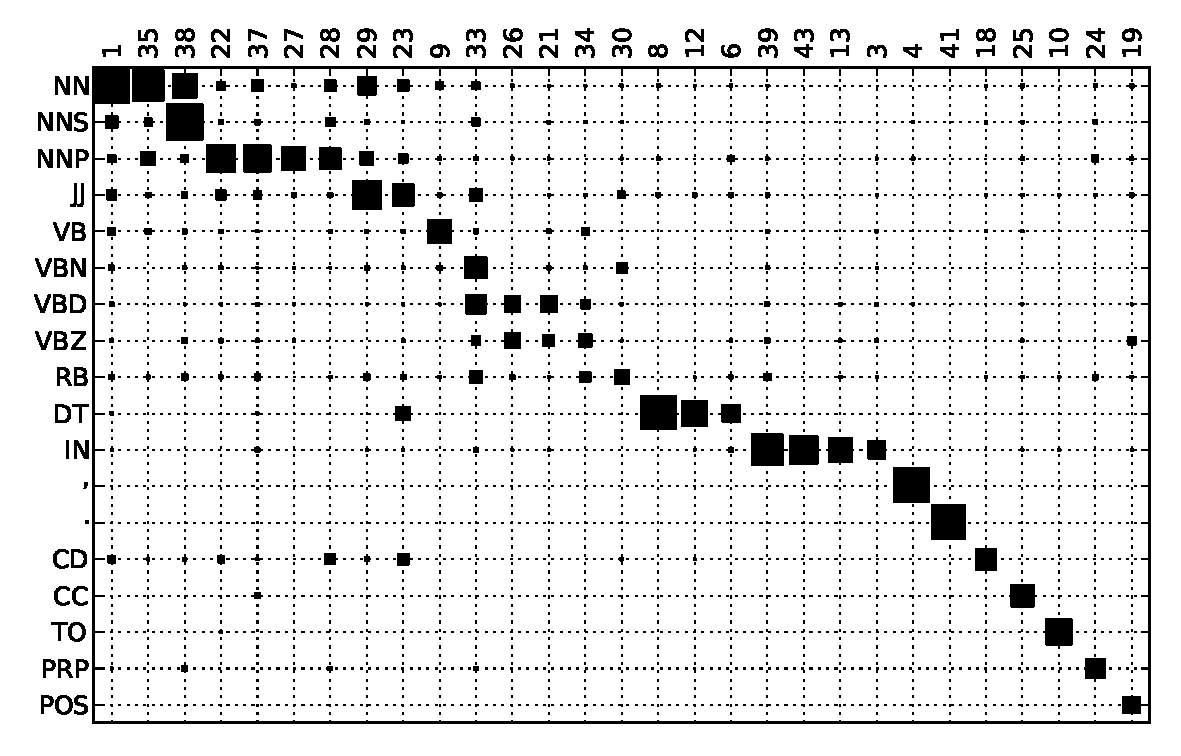
\includegraphics[width=\textwidth]{hinton.eps}
\vspace*{-10mm}
\caption{Hinton diagram of the most frequent tags (rows) and clusters
  (columns).  Area of each square is proportional to the joint
  probability of the given tag and cluster.}
\label{fig:hinton}
\end{figure*}
